\documentclass[tikz,border=12pt]{standalone}
\begin{document}
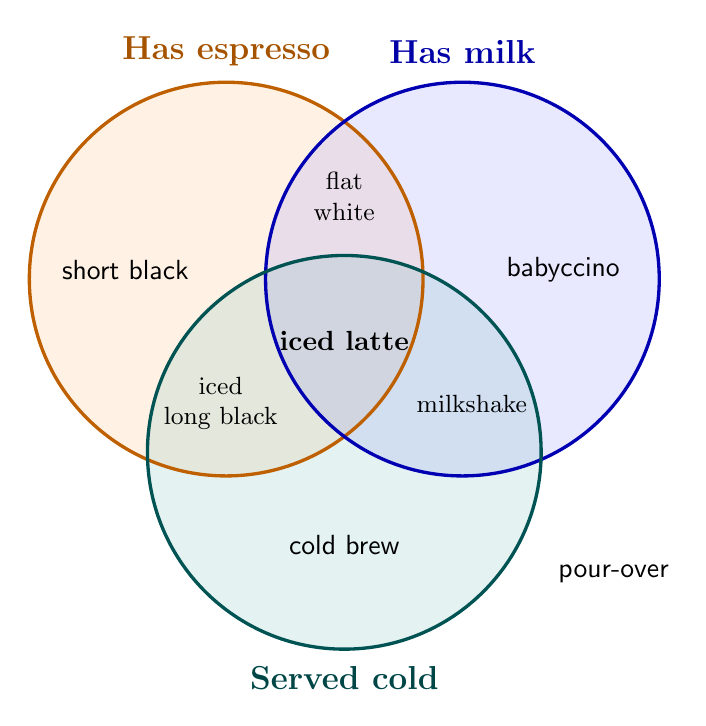
\begin{tikzpicture}[font=\sffamily, every node/.style={align=center}]
  \def\r{2.5}
  % Soft transparent fills make the overlaps visible without obscuring the text.
  \fill[orange!65,opacity=.16] (-1.5,.9) circle (\r);
  \fill[blue!55,opacity=.16] (1.5,.9) circle (\r);
  \fill[teal!65,opacity=.16] (0,-1.3) circle (\r);
  \draw[orange!75!black,very thick] (-1.5,.9) circle (\r);
  \draw[blue!70!black,very thick] (1.5,.9) circle (\r);
  \draw[teal!65!black,very thick] (0,-1.3) circle (\r);

  \node[font=\bfseries\large,orange!65!black] at (-1.5,3.79) {Has espresso};
  \node[font=\bfseries\large,blue!65!black] at (1.5,3.79) {Has milk};
  \node[font=\bfseries\large,teal!55!black] at (0,-4.16) {Served cold};

  \node at (-2.78,1.02) {short black};
  \node at (2.78,1.02) {babyccino};
  \node[font=\small] at (0,1.95) {flat\\white};
  \node[font=\small] at (-1.57,-.68) {iced\\long black};
  \node[font=\small] at (1.62,-.68) {milkshake};
  \node[font=\bfseries] at (0,.12) {iced latte};
  \node at (0,-2.47) {cold brew};
  \node at (3.42,-2.84) {pour-over};
\end{tikzpicture}
\end{document}
